\documentclass{assignment}
\UsingEnglish
\ProjectInfos*{Intro to Communication System}{EE140}{Fall, 2020}{Assignment 5}{Due time : 10:15, Oct 23, 2020 (Friday)}{陈稼霖}{45875852}
\begin{document}
\begin{prob}[Definition of FM, 10pts]
    An FM modulator has output $x_c(t)=10\cos[2\pi f_ct+2\pi f_d\int_0^tm(\tau)\,\mathrm{d}\tau]$, where $f_d=20$ Hz/Volt. Assume that $m(t)=3\Lambda\left(\frac{1}{3}(t-3)\right)$, as shown in Figure \ref{A-5-P-1}.
    \begin{figure}[h]
        \centering
        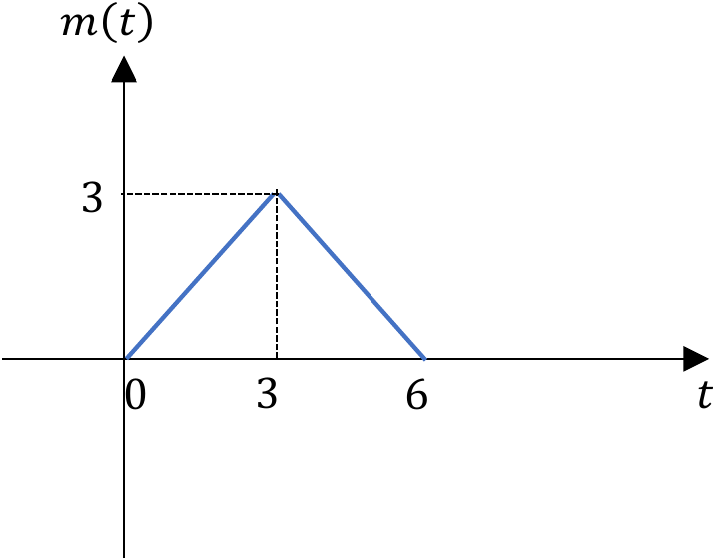
\includegraphics[width=.5\columnwidth]{Assignment-5-Problem-1.png}
        \caption{}
        \label{A-5-P-1}
    \end{figure}
    \begin{itemize}
        \item[1)] Determine the phase deviation in radians.
        \item[2)] Determine the frequency deviation in hertz.
        \item[3)] Determine the peak frequency deviation in hertz.
        \item[4)] Determine the peak phase deviation in radians.
    \end{itemize}
\end{prob}
\begin{sol}
    \begin{itemize}
        \item[1)] The phase deviation in radians is
        \begin{align}
            \phi(t)=&2\pi f_d\int_0^tm(\tau)\,\mathrm{d}\tau=40\pi\int_0^t3\Lambda\left(\frac{1}{3}(\tau-3)\right)\,\mathrm{d}\tau=\left\{\begin{array}{ll}
                20\pi t^2,&0\leq t\leq 3,\\
                -20\pi t^2+240\pi t-360\pi,&3<t\leq 6,\\
                360\pi,&t>6.
            \end{array}\right.\quad(\text{unit: rad})
        \end{align}
        \item[2)] The frequency deviation in hertz is
        \begin{align}
            \frac{1}{2\pi}\frac{\mathrm{d}\phi}{\mathrm{d}t}=&\frac{1}{2\pi}\frac{\mathrm{d}\left[2\pi f_d\int_0^tm(\tau)\,d\tau\right]}{\mathrm{d}t}=f_dm(t)=60\Lambda\left(\frac{1}{3}(t-3)\right)\quad(\text{unit: Hz}).
        \end{align}
        \item[3)] The peak frequency deviation in hertz is
        \begin{align}
            \Delta f=\max\left[\abs{\frac{1}{2\pi}\frac{\mathrm{d}\phi}{\mathrm{d}t}}\right]=60\text{ Hz}.
        \end{align}
        \item[4)] The peak phase deviation in radians is
        \begin{align}
            \Delta\phi=\max[\abs{\phi(t)}]=360\pi\text{ rad}.
        \end{align}
    \end{itemize}
\end{sol}

\begin{prob}[Definition of PM, 10pts]
    A PM modulator has output $x_c(t)=10\cos[2\pi f_ct+k_pm(t)]$, where $k_p=20$ radian/Volts. Assume that $m(t)=3\Lambda\left(\frac{1}{3}(t-3)\right)$, as shown in Figure \ref{A-5-P-1}.
    \begin{itemize}
        \item[1)] Determine the phase deviation in radians.
        \item[2)] Determine the frequency deviation in hertz.
        \item[3)] Determine the peak frequency deviation in hertz.
        \item[4)] Determine the peak phase deviation in radians.
    \end{itemize}
\end{prob}
\begin{sol}
    \begin{itemize}
        \item[1)] The phase deviation in radians is
        \begin{align}
            \phi(t)=k_pm(t)=60\Lambda\left(\frac{1}{3}(t-3)\right)\quad\text{ (unit: rad)}.
        \end{align}
        \item[2)] The frequency deviation in hertz is
        \begin{align}
            \frac{1}{2\pi}\frac{\mathrm{d}\phi}{\mathrm{d}t}=\left\{\begin{array}{ll}
                \frac{30}{\pi},&0\leq t\leq 3,\\
                -\frac{30}{\pi},&3< t\leq 6,\\
                0,&t>6.
            \end{array}\right.(\text{unit: Hz})
        \end{align}
        \item[3)] The peak frequency deviation in hertz is
        \begin{align}
            \Delta f=\max\left[\abs{\frac{1}{2\pi}\frac{\mathrm{d}\phi}{\mathrm{d}t}}\right]=\frac{30}{\pi}\text{ Hz}.
        \end{align}
        \item[4)] The peak phase deviation in radians is
        \begin{align}
            \Delta\phi=\max[\abs{\phi(t)}]=60\text{ rad}.
        \end{align}
    \end{itemize}
\end{sol}

\begin{prob}
    An FM modulator has $f_c=2000$ Hz and $f_d=20$ Hz/Volt. The modulating message signal is $m(t)=5\cos 20\pi t$.
    \begin{itemize}
        \item[1)] What's the peak frequency deviation?
        \item[2)] What's the modulation index?
        \item[3)] Is this narrow band FM? Why?
        \item[4)] If the same $m(t)$ is used for a phase modulator, what must $k_p$ be to yield the modulation index given in 1)?
        \item[5)] Determine the approximate bandwidth of the FM signal, using Carson's rule.
        \item[6)] Determine the bandwidth by transmitting only those side frequencies whose amplitude exceed $1$ percent of the unmodulated carrier amplitude. Use the Table from Page 163 for this calculation. (Hint: find $n_{\max}$, which is the largest value of the integer that satisfies the requirement $J_n(\beta)>0.01$. Then $B=2n_{\max}f_m$.)
        \item[7)] Repeat your calculation in 5), assuming that the amplitude of the modulating signal $m(t)$ is doubled. (Hint: $m(t)=10\cos 20\pi t$.)
        \item[8)] Repeat your calculation in 5), assuming that the frequency of the modulating signal $m(t)$ is doubled. (Hint: $m(t)=5\cos 40\pi t$.)
    \end{itemize}
\end{prob}
\begin{sol}
    \begin{itemize}
        \item[1)] The peak frequency deviation is
        \begin{align}
            \Delta f=f_dA_m=20\times 5=100\text{ Hz}.
        \end{align}
        \item[2)] The modulation index is
        \begin{align}
            \beta=\frac{\Delta f}{f_m}=\frac{100}{10}=10.
        \end{align}
        \item[3)] This is \textbf{not} narrow band FM, since narrow band FM requires that $\beta\ll 1$ but this modulation has $\beta=10$.
        \item[4)] If the same $m(t)$ is used for a phase modulator, then the modulation index is
        \begin{align}
            \beta=k_pA_m=5k_p.
        \end{align}
        To yield the same modulation index as in 1), we need
        \begin{align}
            k_p=2.
        \end{align}
        \item[5)] Using Carson's rule, the approximate bandwidth is
        \begin{align}
            B=2(1+\beta)f_m=2\times(1+10)\times 10=220\text{ Hz}.
        \end{align}
        \item[6)] The modulated signal is
        \begin{align}
            x_c(t)=A_c\sum_{n=-\infty}^{+\infty}J_n(\beta)\cos[2\pi(f_c+nf_m)t].
        \end{align}
        The spectrum of modulated signal is
        \begin{align}
            \notag X_c(f)=&\mathscr{F}[x_c(t)]=\frac{A_c}{2}\sum_{n=-\infty}^{+\infty}J_n(\beta)\left[\delta(f-f_c-nf_m)+\delta(f+f_c+nf_m)\right]\\
            =&\frac{A_c}{2}J_0(\beta)[\delta(f-f_c)+\delta(f+f_c)]+A_c\sum_{n=1}^{+\infty}[\delta(f-f_c-nf_m)+\delta(f+f_c+nf_m)].
        \end{align}
        where $\beta=0$ as obtained in 2), the unmodulated carrier amplitude is $\abs{\frac{A_c}{2}J_0(\beta)}$ and the amplitude of side frequency $f_c\pm nf_m$ is $\abs{A_cJ_n(\beta)}$. According to the table from page 163, $\abs{J_0(10)}=0.246$ and $\abs{J_n(10)}>1\%\frac{\abs{J_0(10)}}{2},\forall 0\leq n\leq 16$, so $n_{\max}=16$. The bandwidth is
        \begin{align}
            B=2n_{\max}f_m=320\text{ Hz}.
        \end{align}
        \item[7)] If the amplitude of the modulating signal $m(t)$ is doubled, i.e., $A_m=10$, then the peak frequency deviation is
        \begin{align}
            \Delta f=f_dA_m=200\text{ Hz}.
        \end{align}
        The modulation index is
        \begin{align}
            \beta=\frac{\Delta f}{f_m}=\frac{200}{10}=20.
        \end{align}
        Using Carson's rule, the approximate bandwidth is
        \begin{align}
            B=2(1+\beta)f_m=2\times(1+20)\times 10=420\text{ Hz}.
        \end{align}
        \item[8)] If the frequency of the modulating signal $m(t)$ is doubled, i.e., $f_m=20$, then the peak frequency deviation is still
        \begin{align}
            \Delta f=f_dA_m=100\text{ Hz}
        \end{align}
        The modulating index is
        \begin{align}
            \beta=\frac{\Delta f}{f_m}=\frac{100}{20}=5.
        \end{align}
        Using Carson's rule, the approximate bandwidth is
        \begin{align}
            B=2(1+\beta)f_m=2\times(1+5)\times 20=240\text{ Hz}.
        \end{align}
    \end{itemize}
\end{sol}

\begin{prob}[Bandwidth of Wideband PM, 20pts]
    Consider a PM signal produced by a sinusoidal modulating wave $m(t)=A_m\cos 2\pi f_mt$ using a modulator with a phase deviation constant equal to $k_p$ radians per volt. The unmodulated carrier wave has frequency $f_c$ and amplitude $A_c$.
    \begin{itemize}
        \item[1)] Show that if the maximum phase deviation of the PM signal is much larger than $1$ radian, the bandwidth of the PM signal varies linearly with the modulation frequency $f_m$.
        \item[2)] Compare this characteristic of a wideband PM signal with that of the corresponding wideband FM signal.
    \end{itemize}
\end{prob}
\begin{sol}
    \begin{itemize}
        \item[1)] The phase deviation of the PM signal is
        \begin{align}
            \phi(t)=k_pm(t)=k_pA_m\cos 2\pi f_mt.
        \end{align}
        The frequency deviation of the PM signal is
        \begin{align}
            \frac{1}{2\pi}\frac{\mathrm{d}\phi(t)}{\mathrm{d}t}=-k_pA_mf_m\sin 2\pi f_mt.
        \end{align}
        The peak frequency deviation of the PM signal is
        \begin{align}
            \Delta f=\max\left[\frac{1}{2\pi}\frac{\mathrm{d}\phi(t)}{\mathrm{d}t}\right]=k_pA_mf_m.
        \end{align}
        The bandwidth of the modulating wave is
        \begin{align}
            W=f_m.
        \end{align}
        The deviation ratio of the PM signal is
        \begin{align}
            D=\frac{\Delta f}{W}=k_pA_m.
        \end{align}
        The bandwidth of the PM signal is
        \begin{align}
            B=2(1+D)W=2(1+k_pA_m)f_m.
        \end{align}
        If the maximum phase deviation of the PM signal is much larger than $1$, i.e., $\max\left[\phi(t)\right]=k_pA_m\gg 1$, then
        \begin{align}
            B\approx 2k_pA_mf_m,
        \end{align}
        i.e., the bandwidth of the PM signal varies linearly with the modulation frequency $f_m$.
        \item[2)] For FM signal, using Carson's rule, its bandwidth is
        \begin{align}
            B=2(1+\beta)f_m=2\left(1+\frac{f_d}{f_m}A_m\right)f_m.
        \end{align}
        The phase deviation of the FM signal is
        \begin{align}
            \phi(t)=2\pi\int_0^tf_dm(\tau)\,\mathrm{d}\tau=2\pi \int_0^tf_dA_m\cos 2\pi f_m\tau\,\mathrm{d}\tau=\frac{f_dA_m}{f_m}\sin 2\pi f_mt.
        \end{align}
        If the maximum phase deviation of the FM signal is much larger than $1$, i.e., $\max[\phi(t)]=\frac{f_dA_m}{f_m}\gg 1$, then
        \begin{align}
            B\approx 2f_dA_m,
        \end{align}
        i.e., the bandwidth of the FM varies linearly withe the amplitude of the modulation wave $A_m$.
    \end{itemize}
\end{sol}

\begin{prob}[Generation of Wideband FM Signal, 20pts]
    A narrowband FM has a carrier frequency of $110$ kHz and a deviation ratio of $0.05$. The bandwidth of the modulating signal is $10$ kHz. This narrowband FM signal is used to generate a wideband FM signal with a deviation ratio of $20$ and a carrier frequency of $100$ MHz. We use the Armstrong indirect FM transmitter in Figure \ref{A-5-P-5} to accomplish this. Give the required value of frequency multiplication $n$. Also, fully define the mixer by giving two permissible frequencies for local oscillator, and define the required bandpass filter (the center frequency and the bandwidth using Carson's rule).
    \begin{figure}[h]
        \centering
        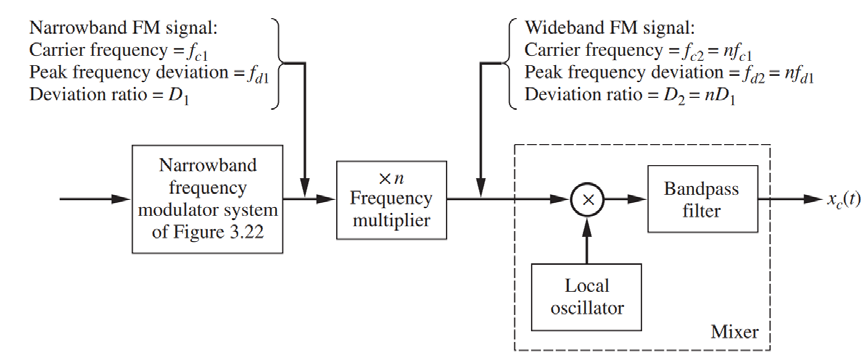
\includegraphics[width=.8\columnwidth]{Assignment-5-Problem-5.png}
        \caption{}
        \label{A-5-P-5}
    \end{figure}
\end{prob}
\begin{sol}
    The narrowband FM signal is
    \begin{align}
        x(t)=A_c\cos[2\pi f_{c1}t+\phi(t)]=A_c\cos[2\pi\cdot 110000t+\phi(t)].
    \end{align}
    The wideband FM signal after frequency multiplier is
    \begin{align}
        y(t)=A_c\cos[2\pi f_{c2}t+n\phi(t)]=A_c\cos[2\pi nf_{c1}t+n\phi(t)]=A_c\cos[2\pi\cdot 110000nt+n\phi(t)].
    \end{align}
    Suppose that the frequency of the local oscillator is $f_{\text{LO}}$. After multiplying with local oscillator, the signal becomes
    \begin{align}
        \notag e(t)=&y(t)\cdot 2\cos 2\pi f_{\text{LO}}t=2A_c\cos[2\pi\cdot 110000nt+n\phi(t)]\cos 2\pi f_{\text{LO}}t\\
        =&A_c\{\cos[2\pi(110000n+f_{\text{LO}})t+n\phi(t)]+\cos[2\pi(110000n-f_{\text{LO}})t+n\phi(t)]\}.
    \end{align}
    To generate a wideband FM signal with a deviation ratio of $20$, we require the value of frequency multiplication $n$ to be
    \begin{align}
        n=\frac{D_2}{D_1}=\frac{20}{0.05}=400.
    \end{align}
    In this way, the signal after multiplying with local oscillator is
    \begin{align}
        e(t)=A_c\{\cos[2\pi(44000000+f_{\text{LO}})t+400\phi(t)]+\cos[2\pi(44000000-f_{\text{LO}})t+400\phi(t)]\}.
    \end{align}
    To generate a wideband FM signal with a carrier frequency of $100$ MHz, we require the frequency of local oscillator to be
    \begin{align}
        f_{\text{LO}}=f_c-f_{c2}=100000000\mathrm{Hz}-44000000\mathrm{Hz}=56000000\mathrm{Hz}=56\mathrm{MHz},
    \end{align}
    or
    \begin{align}
        f_{\text{LO}}=f_c+f_{c2}=100000000\mathrm{Hz}+44000000\mathrm{Hz}=144000000\mathrm{Hz}=144\mathrm{MHz}.
    \end{align}
    The center frequency of the bandpass filter should be $100$ MHz, and according to Carson's rule, its bandwidth should be
    \begin{align}
        B=2(1+D)W=420\mathrm{kHz}.
    \end{align}
    (Actually, the bandwidth within range $[2(1+D)W,f_{c2}-2(1+D)W]=[420\mathrm{kHz},43580\mathrm{kHz}]$ should be OK.)
\end{sol}
\end{document}